\documentclass[12 pt]{book}
\usepackage{amsmath}
\usepackage{amsthm}
\usepackage[paperwidth=5 in,paperheight=5 in,left=7 mm, right=7 mm, top=7 mm, bottom=12 mm]{geometry}
\usepackage{graphics}
\usepackage{fontawesome}
\usepackage{enumitem}
\usepackage{marvosym}
\newcommand{\myitem}{\refstepcounter{enumi}\item[$^\star$\theenumi.]}
\newcommand{\mmyitem}{\refstepcounter{enumi}\item[$^{\star \star}$\theenumi.]}
\setcounter{page}{401}

\usepackage[utf8]{inputenc}
\usepackage{xcolor}
\setlength{\arrayrulewidth}{0.1 mm}
\definecolor{Mycolor2}{HTML}{33cccc}


\usepackage{fancyhdr}

\pagestyle{fancy}
\fancyhf{}
\setlength{\headheight}{10 mm}

\renewcommand{\headrulewidth}{0 mm}


%%----FONT &&& MATHS_FONT----%%

\usepackage{amssymb}
\usepackage{upgreek,xspace}
\newcommand*{\rom}[1]{\expandafter\@\romannumeral #1}

\usepackage[utopia]{mathdesign}
\renewcommand{\familydefault}{\sfdefault}
%\usepackage{newtxtext,newtxmath}
\usepackage[scaled=1]{helvet}
\newcommand*\Times{\fontfamily{ptm}\selectfont}

%%%------PACAKAGES------%%%

\usepackage[letterspace=200]{microtype}
\usepackage{enumitem}
\usepackage{multicol}
\usepackage{pgfplots}
\pgfplotsset{width=8cm,compat=1.16}
\usepackage{tikz}
\usepgfplotslibrary{fillbetween}
\usetikzlibrary{quotes,angles,patterns,through,calc}
\usepgflibrary{arrows.meta}
\usetikzlibrary{optics}
\usetikzlibrary{intersections}

\usetikzlibrary{intersections}

\usepackage[version=4]{mhchem}
\usepackage{chemformula}
\usepackage{elements}

%\DeclareMathSymbol{\shortminus}{\mathbin}{AMSa}{"39}

\usepackage{mathtools}
\usepackage{old-arrows}
\usepackage[b]{esvect}

\newcommand{\midarrow}{\tikz \draw[-Stealth] (0,0) -- +(.1,0);}
\usetikzlibrary{mindmap}
\usetikzlibrary{scopes}
\usetikzlibrary{backgrounds}
\pgfsetlayers{background,main,foreground}
\pgfdeclarelayer{background}
\pgfdeclarelayer{foreground}
\usetikzlibrary{trees}
\usetikzlibrary{shadings}
%\tikzset{every node/.append style = {draw=black,thin}}
\usetikzlibrary{shadows}



\usepackage{color}
\usepackage[autostyle]{csquotes}
\usepackage{xcolor}
\definecolor{Mycolor2}{HTML}{33cccc}
\definecolor{One}{HTML}{336666}
\definecolor{Two}{HTML}{666666}
\definecolor{Three}{HTML}{cc6699}
\definecolor{tomato}{HTML}{FF6347}
\definecolor{darkblue}{HTML}{2c3e50}


\newcommand*\circled[1]{\tikz[thin, baseline=(char.base)]{
            \node[shape=circle,draw,inner sep=1pt] (char) {#1};}}
      

\newcommand{\physics}{\normalsize{\textcolor{black}{\textls*[100]{{\hspace*{75 mm} @10xphysics}}}}}


\newenvironment{my-title}
{
	\begin{center}
	\begin{itshape}
	\large\Times\textit{}
}
{
	\end{itshape}
	\end{center}
}


\newenvironment{definition}
{
	\begin{center}
	\begin{itshape}
	\normalsize\Times\textit{}
}
{
	\end{itshape}
	\end{center}
}


\newenvironment{note}
{
	\begin{center}
	\begin{itshape}
	\normalsize\Times\textit{}
}
{
	\end{itshape}
	\end{center}
}



\begin{document}

\nopagecolor
\boldmath
%\color{white!100}
\Large

%\pagecolor{Mycolor2!80}
%\pagecolor{black!95}
\setlength{\parindent}{0pt}




%%%%   EQUATION-401   %%%%%

\begin{center}
\large{\textls*[100]{\textcolor{white}{REAL OBJECT\\[5 mm]}}}
\end{center}

\begin{center}
\begin{tikzpicture}[use optics,very thick,decoration={
    markings,
    mark=at position 0.3 with {\arrow{Stealth}}}]
\node[mirror,scale=1.75,mirror decoration separation=0.1,mirror decoration amplitude=0.1] at (0,0) {};
\draw (-5,0)--(5,0);
\node at (-4,0) {$\bullet$};
\draw [postaction={decorate}](-4,0)--(0,1)--([turn]150:4);
\draw [put arrow={arrow'=Stealth}](-4,0)--(0,-1)--([turn]-150:4);
\node at (4,0) {$\bullet$};
\draw[dashed] (4,0)--(0,1);
\draw[dashed] (4,0)--(0,-1);
\node at (-4,0)[below]{$O$};
\node at (4,0)[below]{$I$};
\end{tikzpicture}
\end{center}

\large{\Times \textit{Object placed in front of the mirror is called real object.}}




\pagebreak




%%%%   EQUATION-402   %%%%%

\begin{center}
\large{\textls*[100]{\textcolor{white}{VIRTUAL OBJECT\\[5 mm]}}}
\end{center}

\begin{center}
\begin{tikzpicture}[use optics,very thick,decoration={
    markings,
    mark=at position 0.3 with {\arrow{Stealth}}}]
\node[mirror,scale=1.75,mirror decoration separation=0.1,mirror decoration amplitude=0.1] at (0,0) {};
\draw (-5,0)--(5,0);
\node at (-4,0) {$\bullet$};
\draw [postaction={decorate}](-4,0)--(0,1)--([turn]150:4);
\draw [put arrow={arrow'=Stealth}](-4,0)--(0,-1)--([turn]-150:4);
\node at (4,0) {$\bullet$};
\draw[dashed] (4,0)--(0,1);
\draw[dashed] (4,0)--(0,-1);
\node at (-4,0)[below]{$I$};
\node at (4,0)[below]{$O$};
\end{tikzpicture}
\end{center}

\large{\Times \textit{Object placed behind the mirror is called virtual object.}}




\pagebreak



\begin{my-title}
magnification of a mirror
\end{my-title}

%\circled{\textcolor{yellow!95}{\textbf{10}}\textcolor{red!95}{\textbf{X}}}

\begin{center}
\begin{tikzpicture}[use optics,very thick,decoration={
    markings,
    mark=at position 0.15 with {\arrow{Stealth}}}]

\draw (-6,0)--(2.5,0);


\node at (-1.5,0){\tiny{$|$}};
\node at (-3,0){\tiny{$|$}};
\node at (-1.5,0)[below]{\small{$f$}};
\node at (-3,0)[below]{\small{$2f$}};

\draw[ultra thick,-Stealth] (-2.5,0) -- (-2.5,1);
\draw[ultra thick,-Stealth] (-3.95,0) -- (-3.95,-1.55);

\draw[thick,postaction={decorate}] (-2.5,1)--(0.1,1) -- ([turn]212:6);
\draw[thick, postaction={decorate}] (-2.5,1)--(0.25,0) -- ([turn]220:6);

\node[very thick,concave mirror, spherical mirror orientation=ltr,
object height=3.5cm, spherical mirror angle=75,mirror decoration separation=0.075,mirror decoration amplitude=0.07] (M2) at (0,0) {};
\draw[thick] (-4,-3.4) to[dim arrow={label'=$v$}] (0.2,-3.4);
\draw[thick] (-2.5,-2.65) to[dim arrow={label'=$u$}] (0.2,-2.65);
\end{tikzpicture}
\end{center}



\[
m =\dfrac{h_I}{h_O} = - \; \dfrac{v}{u}
\]

\begin{note}
$h_I$ - height of image \quad $h_O$ - height of object \\
$v$ - position of image \quad $u$ - position of object 
\end{note}

\pagebreak




\begin{my-title}
mirror formula
\end{my-title}


\begin{center}
\begin{tikzpicture}[use optics,very thick,decoration={
    markings,
    mark=at position 0.15 with {\arrow{Stealth}}}]

\draw (-6,0)--(2.5,0);
\node at (-1.5,0){\tiny{$|$}};
\node at (-3,0){\tiny{$|$}};
\node at (-1.5,0)[below]{\small{$f$}};
\node at (-3,0)[below]{\small{$2f$}};
\draw[ultra thick,-Stealth] (-2.5,0) -- (-2.5,1);
\draw[ultra thick,-Stealth] (-3.95,0) -- (-3.95,-1.55);
\draw[thick,postaction={decorate}] (-2.5,1)--(0.1,1) -- ([turn]212:6);
\draw[thick, postaction={decorate}] (-2.5,1)--(0.25,0) -- ([turn]220:6);
\node[very thick,concave mirror, spherical mirror orientation=ltr,
object height=3.5cm, spherical mirror angle=75,mirror decoration separation=0.075,mirror decoration amplitude=0.07] (M2) at (0,0) {};
\draw[thick] (-4,-3.4) to[dim arrow={label'=$v$}] (0.2,-3.4);
\draw[thick] (-2.5,-2.65) to[dim arrow={label'=$u$}] (0.2,-2.65);
\end{tikzpicture}
\end{center}


\[
\dfrac{1}{v} + \dfrac{1}{u} =\dfrac{1}{f}
\]

\begin{note}
$v$ - position of image \quad $u$ - position of object \quad $f$ - focal length
\end{note}

\pagebreak


\begin{my-title}
lens formula
\end{my-title}


\begin{center}
\begin{tikzpicture}[use optics,very thick,decoration={
    markings,
    mark=at position 0.15 with {\arrow{Stealth}}}]

\draw (-4.5,0)--(4.5,0);


 \pgfmathsetmacro{\lensRadius}{6}
  \pgfmathsetmacro{\lensHeight}{2}
  \pgfmathsetmacro{\startAngle}{asin(\lensHeight/\lensRadius)}

\draw [ultra thick]  (0,\lensHeight)
  arc[start angle=180-\startAngle,delta angle=2*\startAngle,radius=\lensRadius]
  arc[start angle=-\startAngle,delta angle=2*\startAngle,radius=\lensRadius]
   -- cycle;


\node at (-1.5,0){\tiny{$|$}};
\node at (-3,0){\tiny{$|$}};
\node at (-1.5,0)[below]{\small{$f'$}};
\node at (-3,0)[below]{\small{$2f'$}};
\node at (1.5,0){\tiny{$|$}};
\node at (3,0){\tiny{$|$}};
\node at (1.5,0)[below]{\small{$f$}};
\node at (3,0)[below]{\small{$2f$}};


\draw[ultra thick,-Stealth] (-2.5,0) -- (-2.5,1);
\draw[ultra thick,-Stealth] (3.8,0) -- (3.8,-1.55);
\draw[thick,postaction={decorate}] (-2.5,1)--(0,1) -- ([turn]-33.6:5.5);
\draw[thick, postaction={decorate}] (-2.5,1)--(0,0) -- ([turn]0:5.5);
\draw[thick] (0,-2.75) to[dim arrow={label'=$v$}] (3.8,-2.75);
\draw[thick] (-2.5,-2.75) to[dim arrow={label'=$u$}] (0,-2.75);
\end{tikzpicture}
\end{center}


\[
\dfrac{1}{v} - \dfrac{1}{u} =\dfrac{1}{f}
\]

\begin{note}
$v$ - position of image \quad $u$ - position of object \quad $f$ - focal length
\end{note}

\pagebreak



\begin{my-title}
magnification of a lens
\end{my-title}


\begin{center}
\begin{tikzpicture}[use optics,very thick,decoration={
    markings,
    mark=at position 0.15 with {\arrow{Stealth}}}]

\draw (-4.5,0)--(4.5,0);


 \pgfmathsetmacro{\lensRadius}{6}
  \pgfmathsetmacro{\lensHeight}{2}
  \pgfmathsetmacro{\startAngle}{asin(\lensHeight/\lensRadius)}

\draw [ultra thick]  (0,\lensHeight)
  arc[start angle=180-\startAngle,delta angle=2*\startAngle,radius=\lensRadius]
  arc[start angle=-\startAngle,delta angle=2*\startAngle,radius=\lensRadius]
   -- cycle;


\node at (-1.5,0){\tiny{$|$}};
\node at (-3,0){\tiny{$|$}};
\node at (-1.5,0)[below]{\small{$f'$}};
\node at (-3,0)[below]{\small{$2f'$}};
\node at (1.5,0){\tiny{$|$}};
\node at (3,0){\tiny{$|$}};
\node at (1.5,0)[below]{\small{$f$}};
\node at (3,0)[below]{\small{$2f$}};


\draw[ultra thick,-Stealth] (-2.5,0) -- (-2.5,1);
\draw[ultra thick,-Stealth] (3.8,0) -- (3.8,-1.55);
\draw[thick,postaction={decorate}] (-2.5,1)--(0,1) -- ([turn]-33.6:5.5);
\draw[thick, postaction={decorate}] (-2.5,1)--(0,0) -- ([turn]0:5.5);
\draw[thick] (0,-2.75) to[dim arrow={label'=$v$}] (3.8,-2.75);
\draw[thick] (-2.5,-2.75) to[dim arrow={label'=$u$}] (0,-2.75);
\end{tikzpicture}
\end{center}


\[
m =\dfrac{h_I}{h_O} =  \dfrac{v}{u}
\]

\begin{note}
$h_I$ - height of image \quad $h_O$ - height of object \\
$v$ - position of image \quad $u$ - position of object 
\end{note}

\pagebreak




\begin{my-title}
power of a lens
\end{my-title}


\begin{center}
\begin{tikzpicture}[use optics,very thick,decoration={
    markings,
    mark=at position 0.25 with {\arrow{Stealth}}}]

\draw (-4.5,0)--(4.5,0);


 \pgfmathsetmacro{\lensRadius}{6}
  \pgfmathsetmacro{\lensHeight}{2}
  \pgfmathsetmacro{\startAngle}{asin(\lensHeight/\lensRadius)}

\draw [ultra thick]  (0,\lensHeight)
  arc[start angle=180-\startAngle,delta angle=2*\startAngle,radius=\lensRadius]
  arc[start angle=-\startAngle,delta angle=2*\startAngle,radius=\lensRadius]
   -- cycle;


\node at (1.5,0){\tiny{$|$}};
\node at (1.5,0)[below]{\small{$f$}};

\draw[thick,postaction={decorate}] (-3.5,1)--(0,1) -- ([turn]-33.6:4);
\draw[thick,postaction={decorate}] (-3.5,0.5)--(0,0.5) -- ([turn]-18.75:4);
\draw[thick,postaction={decorate}] (-3.5,-0.5)--(0,-0.5) -- ([turn]18.75:4);
\draw[thick,postaction={decorate}] (-3.5,-1)--(0,-1) -- ([turn]33.6:4);

\end{tikzpicture}
\end{center}


\[
P =\dfrac{1}{f}
\]

\begin{note}
$f$ - focal length in meter
\end{note}

\pagebreak




\begin{my-title}
power of a mirror
\end{my-title}


\begin{center}
\begin{tikzpicture}[use optics,very thick,decoration={
    markings,
    mark=at position 0.25 with {\arrow{Stealth}}}]

\draw (-6,0)--(2.5,0);
\node at (-1.5,0){\tiny{$|$}};
\node at (-1.5,0)[below]{\small{$f$}};

\draw[thick,postaction={decorate}] (-4,1)--(0.1,1) -- ([turn]212:2.5);
\draw[thick, postaction={decorate}] (-4,0.5)--(0.21,0.5) -- ([turn]196:2.5);
\draw[thick,postaction={decorate}] (-4,-1)--(0.1,-1) -- ([turn]148:2.5);
\draw[thick, postaction={decorate}] (-4,-0.5)--(0.21,-0.5) -- ([turn]164:2.5);
\node[very thick,concave mirror, spherical mirror orientation=ltr,
object height=3.5cm, spherical mirror angle=75,mirror decoration separation=0.075,mirror decoration amplitude=0.07] (M2) at (0,0) {};
\end{tikzpicture}
\end{center}


\[
P = - \; \dfrac{1}{f}
\]

\begin{note}
$f$ - focal length in meter
\end{note}

\pagebreak




\begin{my-title}
Snell's Law
\end{my-title}


\begin{center}
\begin{tikzpicture}[use optics,very thick,decoration={
    markings,
    mark=at position 0.25 with {\arrow{Stealth}}}]

\draw[thick] (-4.5,0)--(4.5,0);

\draw[thick] (0,2.75) -- (0,-2.75);
\draw [postaction={decorate}] (-2,2)--(0,0)--(1,-2.5);
\node at (4,-0.5){$\upmu_2$};
\node at (4,2.5){$\upmu_1$};
\draw (0,0.5) arc[start angle=90,delta angle=45,radius=0.5] node[left=-1mm,above]{$i$};

\draw (0,-0.65) arc[start angle=270,delta angle=23,radius=0.65] node[left=1mm,below]{$r$};
\end{tikzpicture}
\end{center}


\[
\dfrac{\sin i}{\sin r} = \dfrac{\upmu_2}{\upmu_1}
\]

\begin{note}
$i$ - angle of incidence \quad $r$ - angle of refraction\\
$\upmu_1, \upmu_2$ - refractive index of medium 1 \& 2
\end{note}

\pagebreak


\begin{my-title}
apparent depth
\end{my-title}


\begin{center}
\begin{tikzpicture}[use optics,very thick,every node/.style={scale=0.75},decoration={
    markings, mark=at position 0.25 with {\arrow{Stealth}}}]

\draw[thick] (4,2.5)--(-4,2.5);
\draw[thick] (-1.5,3.5) -- (-1.5,1.5);
\draw[thick] (1.5,3.5) -- (1.5,1.5);
\draw [postaction={decorate}] (-3,3.75)--(-1.5,2.5)--(0,0)node{$\bullet$} node[below]{$O$};
\draw [postaction={decorate}] (3,3.75)--(1.5,2.5)--(0,0);
\draw [dashed,thick] (-3,3.75)--(-1.5,2.5)--([turn]0:1.95) node{$\bullet$} node[below]{$I$};
\draw [dashed, thick] (3,3.75)--(1.5,2.5)--([turn]0:1.95);
\node at (3.25,1.25){$\upmu$};
\draw[thick] (-1.5,0) to[dim arrow={label'=$h_O$}] (-1.5,2.5);
\draw[thick] (0.5,1.25) to[dim arrow={label'=$h_I$}] (0.5,2.5);
\end{tikzpicture}
\end{center}


\[
h_I =  \dfrac{h_O}{\upmu}
\]

\begin{note}
$h_O$ - depth of object \quad $h_I$ - depth of image\\
$\upmu$ - refractive index of the medium
\end{note}

\pagebreak



\begin{my-title}
Prism
\end{my-title}

\begin{definition}
A prism is a transparent optical element with flat, polished surfaces that refract light. At least two of the flat surfaces must have an angle between them.
\end{definition}

\begin{center}
\begin{tikzpicture}[scale=2, very thick, use optics,very thick,every node/.style={scale=0.75},decoration={
    markings, mark=at position 0.25 with {\arrow{Stealth}}}]

\draw[dashed,thick] (-1,0) -- (0,0.5) edge (0,2.5) -- (1,0);
 \draw (-1,0) rectangle (1,2) -- (0,2.5) -- (-1,2);
\end{tikzpicture}
\end{center}



\pagebreak





\begin{my-title}
refraction through prism
\end{my-title}

\begin{center}
\begin{tikzpicture}[scale=1.35, very thick, use optics,very thick,every node/.style={scale=0.85},decoration={
    markings, mark=at position 0.25 with {\arrow{Stealth}}},dot/.style={name=#1},
 extended line/.style={shorten >=-#1,shorten <=-#1},
  extended line/.default=1cm,one end extended/.style={shorten >=-#1},
 one end extended/.default=1cm]

\draw (0,0) node[dot=A]{}--(4,0) node[dot=C]{}--([turn]120:4) node[dot=B]{} --cycle;
\node [dot=P] at (0.5,1.75){};
\node [dot=Q] at (3.5,1.75){};

\draw [dashed,thick,extended line=1.65 cm] ($(A)!(P)!(B)$) -- (P);
\draw [dashed,thick,extended line=1.65 cm] ($(C)!(Q)!(B)$) -- (Q);

\coordinate (P') at ($(A)!(P)!(B)$);
\coordinate (Q') at ($(C)!(Q)!(B)$);

\draw[thick] (-1,1)node[dot=D]{}--(P') -- (Q') --([turn]-30:2)node[dot=D']{} ;

\draw [dashed,thick] (D) -- ($(P')!-3cm!(D)$) coordinate (E);
\draw [dashed,thick] (D') -- ($(Q')!-0.837cm!(D')$) coordinate (F);

\draw [dashed,thick] (P) -- ($(P')!-1.28cm!(P)$) coordinate (G);
\draw [dashed,thick] (Q) -- ($(Q')!-1.28cm!(Q)$) coordinate (H);

\node at (E) {$\bullet$};
\pic [draw=black,"$\delta$", angle eccentricity=1.45,angle radius=0.8cm] {angle = Q'--F--E};

\pic [draw=black,"$i_1$", angle eccentricity=1.45,angle radius=0.8cm] {angle = P--P'--D};

\pic [draw=black,"$r_1$", angle eccentricity=1.45,angle radius=0.8cm] {angle = G--P'--Q'};

\pic [draw=black,"$r_2$", angle eccentricity=1.45,angle radius=0.8cm] {angle = P'--Q'--H};

\pic [draw=black,"$i_2$", angle eccentricity=1.45,angle radius=0.8cm] {angle = D'--Q'--Q};

\pic [draw=black,"$A$", angle eccentricity=1.45,angle radius=0.8cm] {angle = A--B--C};


\end{tikzpicture}
\end{center}


\[
A = r_1 + r_2
\]
\[
\delta = (i_1 + i_2) - (r_1+r_2)
\]



\pagebreak




\begin{my-title}
refraction through prism
\end{my-title}

\begin{center}
\begin{tikzpicture}[scale=1.4, very thick, use optics,very thick,every node/.style={scale=0.85},decoration={
    markings, mark=at position 0.25 with {\arrow{Stealth}}},dot/.style={name=#1},
 extended line/.style={shorten >=-#1,shorten <=-#1},
  extended line/.default=1cm,one end extended/.style={shorten >=-#1},
 one end extended/.default=1cm]

\draw (0,0) node[dot=A]{}--(4,0) node[dot=C]{}--([turn]120:4) node[dot=B]{} --cycle;
\node [dot=P] at (0.5,1.75){};
\node [dot=Q] at (3.5,1.75){};

\draw [dashed,thick,extended line=1.65 cm] ($(A)!(P)!(B)$) -- (P);
\draw [dashed,thick,extended line=1.65 cm] ($(C)!(Q)!(B)$) -- (Q);

\coordinate (P') at ($(A)!(P)!(B)$);
\coordinate (Q') at ($(C)!(Q)!(B)$);
\node at (P')[above]{$P$};
\node at (Q')[below]{$Q$};

\draw[thick] (-1,1)node[dot=D]{}--(P') -- (Q') --([turn]-30:2)node[dot=D']{} ;

\draw [dashed,thick] (D) -- ($(P')!-3cm!(D)$) coordinate (E);
\draw [dashed,thick] (D') -- ($(Q')!-0.837cm!(D')$) coordinate (F);

\draw [dashed,thick] (P) -- ($(P')!-1.28cm!(P)$) coordinate (G);
\draw [dashed,thick] (Q) -- ($(Q')!-1.28cm!(Q)$) coordinate (H);

\node at (G)[below]{$O$};
\node at (F)[above]{$F$};

\node at (E) {$\bullet$};
\pic [draw=black,"$\delta$", angle eccentricity=1.45,angle radius=0.8cm] {angle = Q'--F--E};

\pic [draw=black,"$i_1$", angle eccentricity=1.45,angle radius=0.8cm] {angle = P--P'--D};

\pic [draw=black,"$r_1$", angle eccentricity=1.45,angle radius=0.8cm] {angle = G--P'--Q'};

\pic [draw=black,"$r_2$", angle eccentricity=1.45,angle radius=0.8cm] {angle = P'--Q'--H};

\pic [draw=black,"$i_2$", angle eccentricity=1.45,angle radius=0.8cm] {angle = D'--Q'--Q};

\pic [draw=black,"$A$", angle eccentricity=1.45,angle radius=0.8cm] {angle = A--B--C};


\end{tikzpicture}
\end{center}

\begin{note}
$A$ - angle of prism, \quad $\delta$ - deviation, \quad $\upmu$ - refractive index
\end{note}

\pagebreak

\begin{note}
\begin{align*}
\textit{In quadrilateral APOQ}, \\ 
\angle A + \angle P + \angle O + \angle Q &= 360^\circ \\
A + 90^\circ + \angle O + 90^\circ &= 360^\circ \\
A  + \angle O  &= 180^\circ \\
A  &= 180^\circ - \angle O \quad \cdots (1) \\[8 mm]
\textit{In triangle POQ}, \\ 
r_1 + \angle O + r_2 &= 180^\circ \\
r_1 + r_2 &= 180^\circ - \angle O  \quad \cdots (2) \\[8 mm]
\textit{From (1) \& (2) we have}, \\
A &= r_1 + r_2
\end{align*}
\end{note}


\pagebreak

\begin{note}
\begin{align*}
\textit{In triangle PQF}, \\[2 mm]
\delta &= (i_1 - r_1 ) + (i_2 - r_2)  \\[2 mm]
\delta &= (i_1 + i_2) - (r_1+r_2)  \\[2 mm]
\delta &= (i_1 + i_2) - A
\end{align*}
\end{note}


\pagebreak

\begin{note}
\begin{align*}
\textit{For small angled prism}, \\[2 mm]
\textit{from refration at point P, we have} \\[2 mm]
\dfrac{\sin i_1}{\sin r_1} &= \upmu \\[2 mm]
i_1 &= \upmu \; r_1\\
\textit{from refration at point Q, we have} \\[2 mm]
\dfrac{\sin r_2}{\sin i_2} &= \dfrac{1}{\upmu}  \\[2 mm]
i_2 &= \upmu \; r_2
\end{align*}
\end{note}


\pagebreak

\begin{note}
\begin{align*}
\delta &= (i_1 + i_2) - A \\[2 mm]
\delta &= (\upmu \; r_1 + \upmu \; r_2) - A \\[2 mm]
\delta &= \upmu \; (r_1 + r_2) - A \\[2 mm]
\delta &= \upmu \; A - A \\[2 mm]
\delta &= \left( \upmu - 1 \right) A 
\end{align*}
\end{note}

\begin{my-title}
deviation for small angled prism\\[-25 mm]
\end{my-title}
\[
\delta = \left( \upmu -1 \right) A
\]

\pagebreak





\begin{my-title}
angular dispersion
\end{my-title}
{\physics}
\begin{center}
\begin{tikzpicture}[scale=1.4, very thick, use optics,very thick,every node/.style={scale=0.85},decoration={
    markings, mark=at position 0.25 with {\arrow{Stealth}}},dot/.style={name=#1},
 extended line/.style={shorten >=-#1,shorten <=-#1},
  extended line/.default=1cm,one end extended/.style={shorten >=-#1},
 one end extended/.default=1cm]

\draw (0,0) node[dot=A]{}--(4,0) node[dot=C]{}--([turn]120:4) node[dot=B]{} --cycle;
\node [dot=P] at (0.5,1.75){};
\node [dot=Q] at (3.5,1.75){};

\coordinate (P') at ($(A)!(P)!(B)$);
\coordinate (Q') at ($(C)!(Q)!(B)$);

\draw[thick] (-1,1)--(P');

\draw (0,0)--(4,0)--([turn]120:1.5) coordinate (x);
\draw (0,0)--(4,0)--([turn]120:1.75) coordinate (y);
\draw (0,0)--(4,0)--([turn]120:2) coordinate (z);


\draw[thick] (P') -- (x) --([turn]-20:2) coordinate (x') node[right]{\Times{\textit{violet}}};
\draw[thick] (P') -- (y) --([turn]-20:2) coordinate (y') node[right]{\Times{\textit{yellow}}};
\draw[thick] (P') -- (z) --([turn]-20:2) coordinate (z') node[right]{\Times{\textit{red}}};

\draw [dashed,thick] (D) -- ($(P')!-4cm!(D)$) coordinate (o');

\draw [dashed,thick] (x') -- ($(x)!-1.34cm!(x')$) coordinate (x'');
\draw [dashed,thick] (y') -- ($(y)!-1.15cm!(y')$) coordinate (y'');
\draw [dashed,thick] (z') -- ($(z)!-0.85cm!(z')$) coordinate (z'');

\node at (o') {$\bullet$};

\pic [thick,draw=black,"$\delta_v$", angle eccentricity=1.1,angle radius=3cm] {angle = x'--x''--o'};
\pic [thick,draw=black,"$\delta_y$", angle eccentricity=1.15,angle radius=2.3cm] {angle = y'--y''--o'};
\pic [thick,draw=black,"$\delta_r$", angle eccentricity=1.2,angle radius=1.5cm] {angle = z'--z''--o'};

\end{tikzpicture}
\end{center}

\begin{my-title}
\[
 \textit{angular dispersion} \; = \; \left( \delta_v - \delta_r \right)
\]
\end{my-title}



\pagebreak




\begin{my-title}
number of images
\end{my-title}


{\physics}

\begin{center}
\begin{tikzpicture}[scale=0.9,use optics,very thick,decoration={
    markings,
    mark=at position 0.3 with {\arrow{Stealth}}}]
\draw[thick,decorate,decoration={border,angle=45 ,amplitude=-0.25cm, segment length=0.25cm}] (0,0)--(5,0);
\draw[very thick] (0,0) coordinate (a) --(5,0) coordinate (b);
\begin{scope}[rotate=45]
\draw[thick,decorate,decoration={border,angle=130 ,amplitude=0.25cm, segment length=0.25cm}] (0,0)--(5,0);
\draw[very thick] (0,0) coordinate (a) --(5,0) coordinate (c);
\end{scope}
\pic [draw=black,"$\theta$", angle eccentricity=1.45,angle radius=0.8cm] {angle = b--a--c};
\node at (2.5,2.75*sin 22) {$\bullet$};
\end{tikzpicture}
\end{center}

\[
\dfrac{360^\circ}{\theta} = N
\]

\begin{note}
\begin{itemize}
\item If $N$ is even integer then number of images $n=N-1$ \\
\item If $N$ is odd integer then number of images $n=N$ \\
\item If $N$ is odd integer and object is on the bisector of mirrors then number of images $n=N-1$ \\
\end{itemize}
\end{note}


\pagebreak
%
%\begin{note}
%\begin{tikzpicture}
%[edge from parent fork down, sibling distance=30mm, level distance=15mm,
%every node/.style={draw,red,line width=0.75,rounded corners},
%edge from parent/.style={red,line width=0.75,draw,line cap=round}] 
%\node {n (number of images)}
%      child {node {$n=N-1$} child {node {even integer}}}
%      child {node {$n=N$} child {node {odd integer}} }
%      child {node {$n=N-1$}}
%      child {node {$n=[ N ]$}};
%\end{tikzpicture}
%\end{note}


\pagebreak





\begin{tikzpicture}
\draw (-2,0) -- (2,0);
\filldraw [gray] (0,0) circle (2pt);
\draw (-2,-2) .. controls (0,0) .. (2,-2);
\draw (-2,2) .. controls (-1,0) and (1,0) .. (2,2);
\end{tikzpicture}
 aaa

\end{document}